\subsection{Results}

In this study, participants had an average of 2.9 target sites enabled. They visited at least one target site 71\% of days on average. On each of those days, participants experienced interventions an average of 6.6 times.

% \subsection{RQ5: Does improving users' mental model by reminding them of how the system works when presenting a new intervention help reduce attrition?}

\begin{figure}[tb]
\centering
	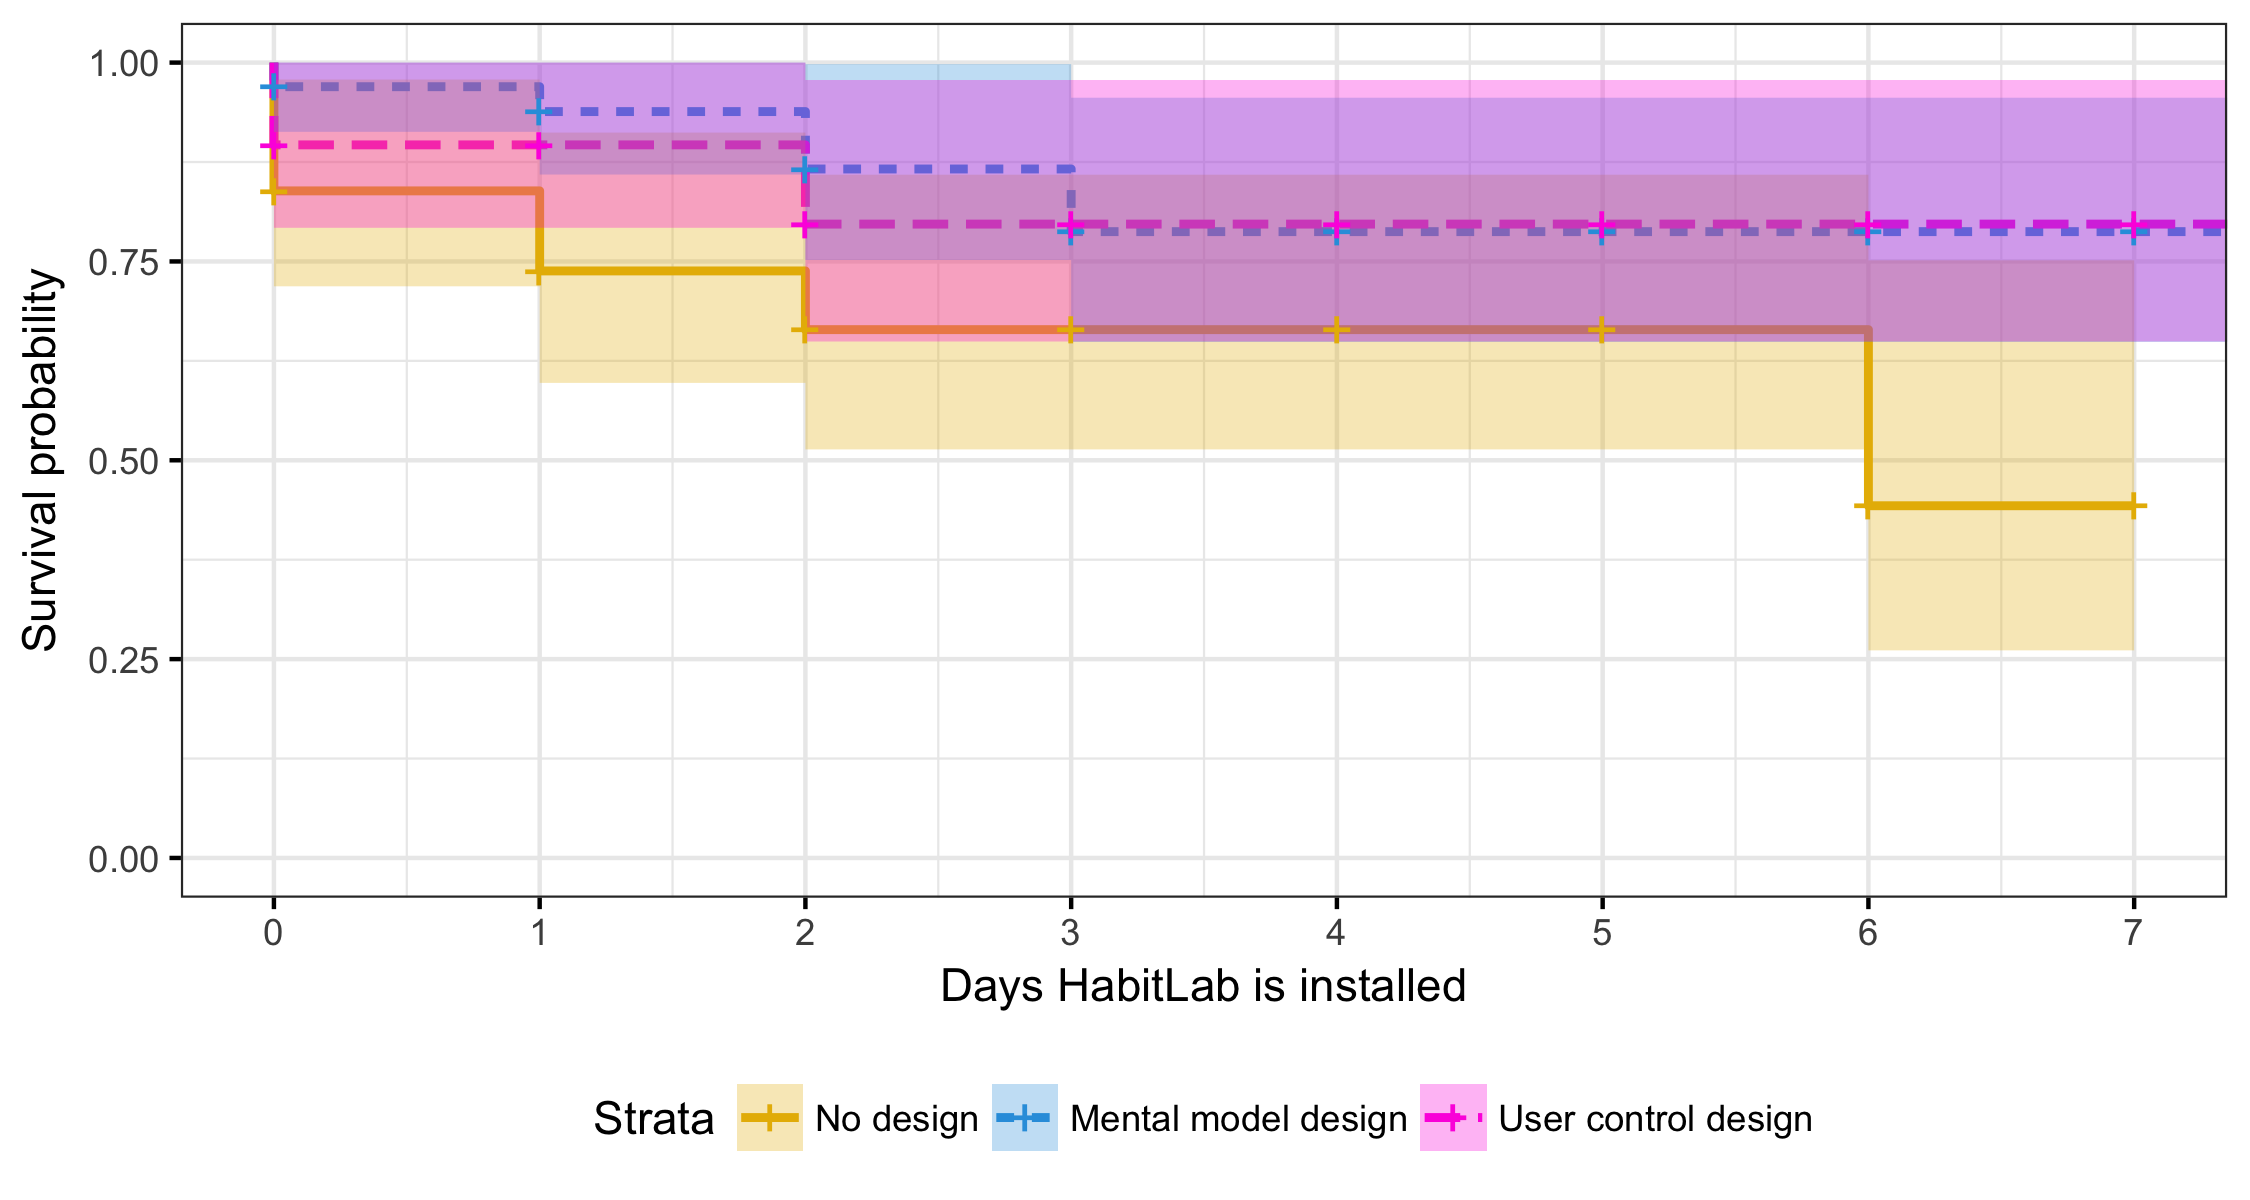
\includegraphics[width=1.0\textwidth]{figures/none_vs_info.png}
	\caption{Reminding users about how the rotations worked every time a new intervention was introduced significantly reduced attrition rates.}
\label{fig:attrition_none_vs_info}
\end{figure}

% Table created by stargazer v.5.2 by Marek Hlavac, Harvard University. E-mail: hlavac at fas.harvard.edu
% Date and time: Thu, Apr 19, 2018 - 09:03:30
\begin{table}[tb] \centering 
  \caption{A Cox proportional hazards analysis suggests that the informational intervention that corrected users' mental models was successful in reducing attrition due to rotation. Coefficients are log hazard ratio.} 
  \label{tab:cox_regression_design} 
\begin{tabular}{@{\extracolsep{5pt}}lc} 
\\[-1.8ex]\hline 
\hline \\[-1.8ex] 
 & \multicolumn{1}{c}{\textit{Dependent variable:}} \\ 
\cline{2-2} 
\\[-1.8ex] & Log hazard ratio \\ 
\hline \\[-1.8ex] 
 Mental model design & $-$1.015$^{*}$ \\ 
  & (0.494) \\ 
  User control design & $-$0.869 \\ 
  & (0.527) \\ 
 \hline \\[-1.8ex] 
Observations & 93 \\ 
\hline 
\hline \\[-1.8ex] 
\textit{Note:}  & \multicolumn{1}{r}{$^{*}$p$<$0.05; $^{**}$p$<$0.01; $^{***}$p$<$0.001} \\ 
\end{tabular} 
\end{table} 

% \subsection{RQ6: Does improving users' sense of control by allowing them to opt-out of seeing a newly introduced intervention in the future help reduce attrition?}

The Cox proportional hazard regression indicates that the mental model design  significantly reduces attrition rates relative to no design ($p < 0.05$, Figure~\ref{fig:attrition_none_vs_info}, Table~\ref{tab:cox_regression_design}). This result supports H\ref*{hyp:mentalmodel}. % After 2 days, 94\% of participants in the mental model condition remain, while 82\% remain in the user control condition and only 72\% remain in the no design (control) condition. Adding the additional option to permanently turn off the intervention the first time it is seen does not significantly change attrition rates, relative to simply informing the user that rotation is happening. % 7 days
After seven days, 79\% of participants in the mental model condition remain, while 80\% remain in the user control condition and only 44\% remain in the no design (control) condition. In other words, the intervention coditions more than halved the attrition rate, from 56\% to 21\% attrition. Adding the additional option to permanently turn off the intervention the first time it is seen is not significantly different from no design given our sample size. % It appeared to perform similarly to the mental model condition (Figure~\ref{fig:attrition_none_vs_info}), but had larger variance, thus the lack of statistical significance. This result indicates that H\ref*{hyp:control} was not supported.

There was no effect of condition on effectiveness: the full model was not significantly more explanatory than the reduced model without the condition variable ($\chi^{2}(2) = 1.46, n.s.$). So, these interventions did not reduce effectiveness while they were improving attrition. %Showing the designs had no effect on daily time spent per domain, using the same analysis from Study 1, as shown in Table~\ref{tab:designs_timespent_noeffect}. % 7 days

% In sum, adding an information intervention reduced attrition by more than a half, from 56\% to 21\% attrition. % \msb{TODO: change all these numbers to seven days, to match the graphs} \geza{done}

% \msb{TODO: support or not support H4, H5}

% \msb{TODO: ideally, report whether the interventions impacted effectiveness} \gezacomment{done}

% Table created by stargazer v.5.2 by Marek Hlavac, Harvard University. E-mail: hlavac at fas.harvard.edu
% Date and time: 三, 4月 18, 2018 - 22时28分14秒
% \begin{table}[tb] \centering 
%   \caption{Daily time spent on sites in the no design, mental model, and user control conditions. There was no significant difference in time spent between conditions.} 
%   \label{tab:designs_timespent_noeffect} 
% \begin{tabular}{@{\extracolsep{5pt}}lc} 
% \\[-1.8ex]\hline 
% \hline \\[-1.8ex] 
%  & \multicolumn{1}{c}{\textit{Dependent variable:}} \\ 
% \cline{2-2} 
% \\[-1.8ex] & Log time spent per day \\ 
% \hline \\[-1.8ex] 
%  Mental model (baseline: no design) & $-$0.170 \\ 
%   & (0.191) \\ 
%   User control & 0.042 \\ 
%   & (0.186) \\ 
%   Constant & 4.554$^{***}$ \\ 
%   & (0.198) \\ 
%  \hline \\[-1.8ex] 
% Observations & 1,041 \\ 
% \hline 
% \hline \\[-1.8ex] 
% \textit{Note:}  & \multicolumn{1}{r}{$^{*}$p$<$0.05; $^{**}$p$<$0.01; $^{***}$p$<$0.001} \\ 
% \end{tabular} 
% \end{table} 

% \begin{figure}[tb]
% \centering
% 	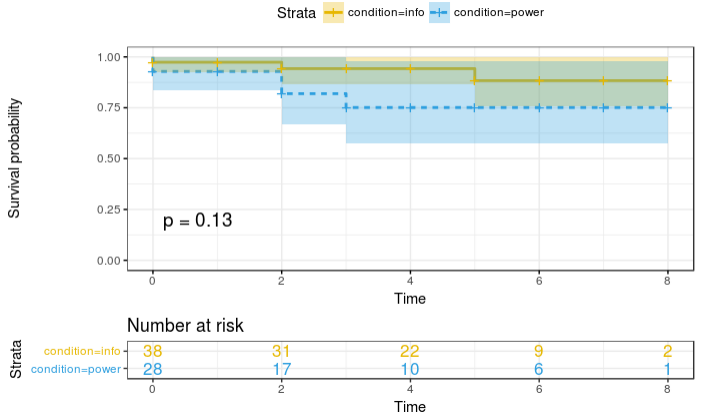
\includegraphics[width=1.0\textwidth]{figures/info_vs_power.png}
% 	\caption{Adding an option to permanently turn off the intervention to our design did not change attrition rates relative to simply showing information.}
% \label{fig:attrition_info_vs_power}
% \end{figure}

